\section{Comparison with Related Work}
In the last chapter, we have demonstrated that our grammar-based evolutionary search method has the capability discover multigrid methods of novel structure and which, in certain cases, yield faster solvers compared to all known multigrid cycles.
Furthermore, by applying the generalization procedure presented in  Section~\ref{sec:generalization}, we were able to evolve multigrid methods that achieve a high degree of efficiency over a set of increasingly-difficult instances of the same problem, while, in certain cases, these methods can even be generalized to larger problem instances than considered within their evolution.
However, since the application of artificial intelligence and optimization methods to the solution of PDEs includes a wide range of different methods and approaches, it is important to categorize the approach presented in this thesis within this growing field.
We can classify AI-based methods for solving PDEs according to different criteria.
\begin{figure}
	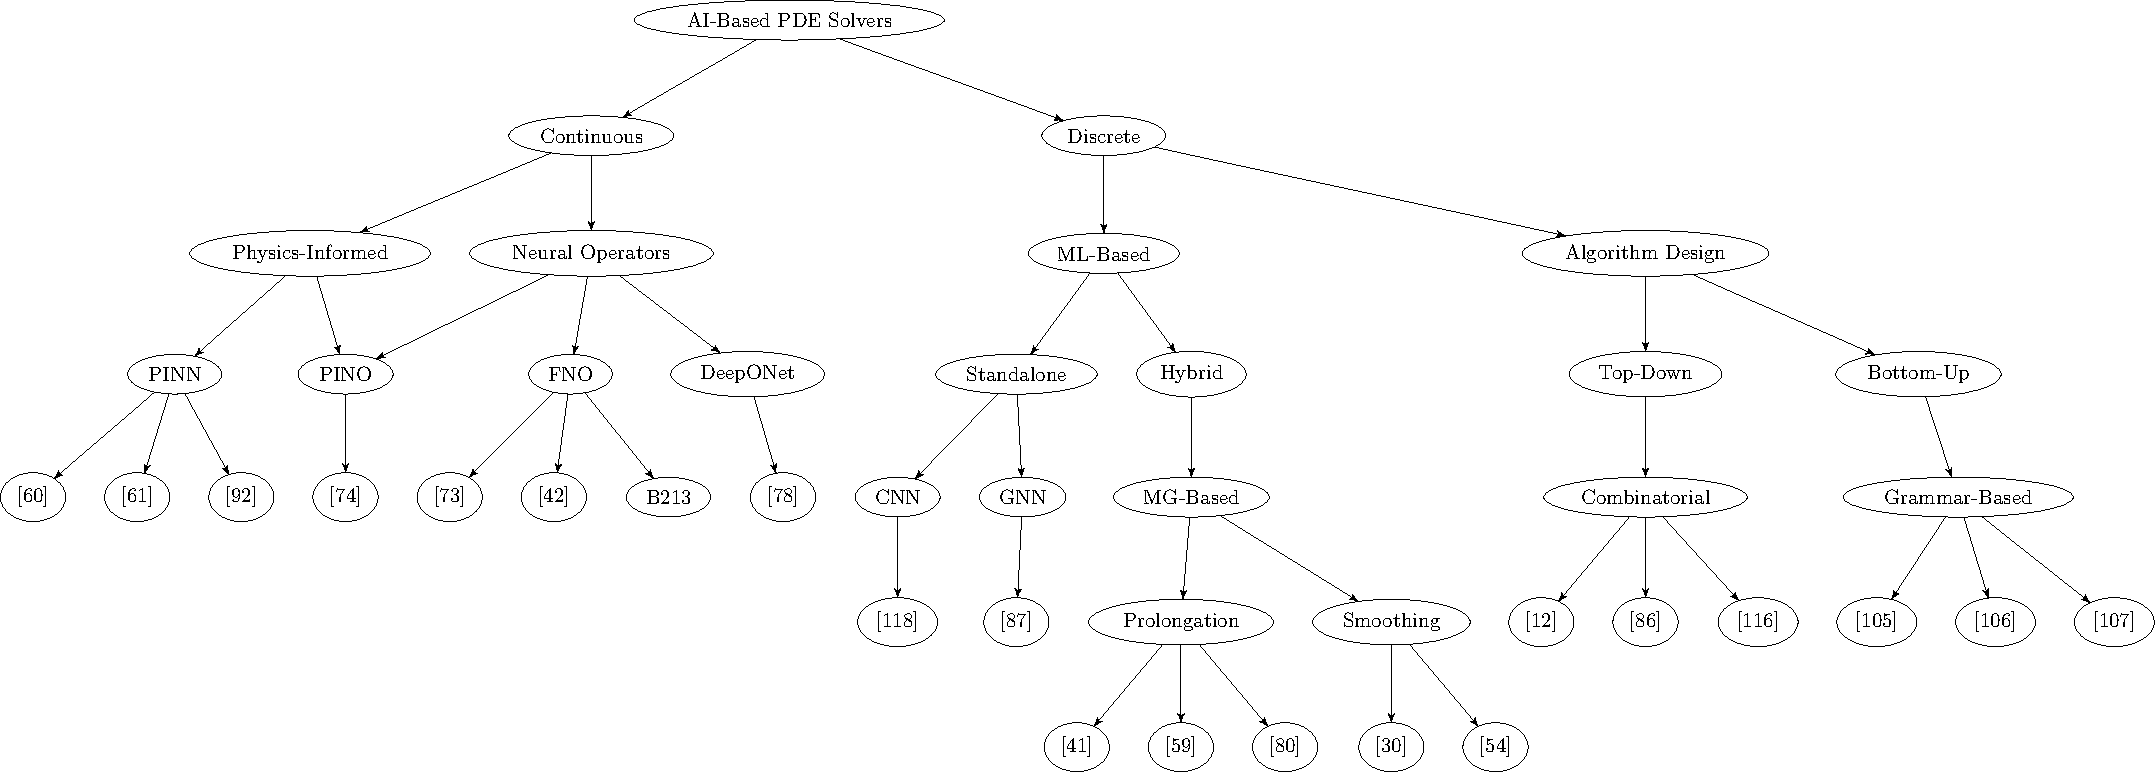
\includegraphics[width=\textwidth]{figures/trees/related_work.pdf}
	\caption{}
	\label{}
\end{figure}
First of all, we can distinguish methods that aim to solve a PDE directly in the continuous domain and, those that require it to be formulated as a discrete problem, usually obtained by applying a specific discretization method.
The currently most popular machine learning-based methods, physics-informed neural networks~\cite{karniadakis2021physics,raissi2019physics,kharazmi2019variational,kharazmi2021hp} and neural operators~\cite{li2020fourier,guibas2021efficient,lu2021learning,li2021physics}, fall into the former category.
This class of methods aims to learn the function that represents solution or the operator of a given PDE by utilizing the fact that neural networks can act as universal function approximators when given enough data~\cite{hornik1989multilayer}.
Physics-informed methods try to improve upon purely data-driven methods by directly incorporating the physical constraints of the given PDE into the learning process.
Neural operators aim to achieve a higher degree of generalization by learning a representation of the operator of a PDE instead of approximating its solution.
Recently, the usability of machine learning-based methods has been tremendously improved through the availability of easy-to-use and well-maintained implementations, such as DeepXDE~\cite{lu2021deepxde} and NVIDIA Modulus~\cite{hennigh2021nvidia}. 
Instead of directly targeting a PDE in the continuous domain, the second branch of AI-based methods operate on its discrete version obtained after applying a suitable discretization method.
Therefore, these methods can either act as a direct replacement for classical numerical solvers or operate in combination with them.
An early example for the former is the neural network-based PDE solvers proposed by Lagaris et al.~\cite{lagaris1998artificial} but also more recent approaches based on convolutional~\cite{thuerey2020deep} and graph neural networks~\cite{pfaff2020learning} fall into this category.
In contrast, AI-based methods that work in combination with existing solvers do not try to replace the method as a whole but rather aim to enhance it, for instance, by adding or replacing certain steps of the method or by finding an optimal configuration for each of its parameters and design options.
Multigrid methods are an often-considered target since these methods have the potential to achieve an optimal asymptotic complexity while possessing a large number of configuration options and complex interactions between each of its components.
A first towards the automated design of an optimal multigrid method has been the work by Oosterlee and Wienands~\cite{oosterlee2003genetic}, which uses a genetic algorithm to optimize the choice of each multigrid component.
Similarly, Thekale et al.~\cite{thekale2010optimizing} aim to optimize the number of multigrid cycles within a full-multigrid method using a branch-and-bound approach, while Brown et al.~\cite{brown2021tuning} optimize the algorithmic parameters of a two-grid method by solving a minimax problem obtained from a LFA-based analysis.
All these works have in common that they are based on the classical formulation of multigrid methods, as shown in Algorithm~\ref{alg:multigrid-cycle}.
As their optimization capabilities are still restricted to a set of global algorithmic parameters, they can be classified as top-down algorithm design methods.
In contrast, as we have shown in this work, expressing each possible computational step of multigrid method as a separate production rule of a context-free grammar allows us to treat the task of designing an optimal multigrid method as a program synthesis.
Therefore, according to our classification of algorithm design methods in Chapter~%TODO insert ref her
our work can be considered as the first implementation of a bottom-up approach for automated multigrid design.
However, while our approach offers the flexibility to construct arbitrary sequences of multigrid operations on a given hierarchy of discretizations, similar to~\cite{oosterlee2003genetic,thekale2010optimizing,brown2021tuning} we consider the internal structure of each individual operation as immutable.
Recently, ML-based methods have been utilized to enhance or replace certain operations within a multigrid method.
A first example are the works by Katrutsa et al.~\cite{katrutsa2020black}, Greenfeld et al.~\cite{greenfeld2019learning} and Luz et at.~\cite{luz2020learning} which utilizes ML-methods to learn optimized prolongation operators.
Huang et al.~\cite{huang2021learning} and Fanaskov~\cite{fanaskov2021neural} apply a similar approach to the optimization of smoothers.
The works by Taghibakhshi et al.~\cite{taghibakhshi2021optimization} and Markidis~\cite{markidis2021old} go even one step further.
In the former the authors replace the coarsening step within an algebraic multigrid method altogether by a machine learning system, while in~\cite{markidis2021old} the author proposes to employ a physics-informed neural network as a coarse-grid solver.
Finally, Hsieh et al.~\ref{hsieh2019learning} take a different direction by enhancing the approximation obtained in each step of an iterative solver in an additional neural network-based correction phase.
Since these ML-based methods all focus on the optimization of the individual components of a multigrid method but consider the methods algorithmic structure as immutable, they can be considered as a complementary approach to the algorithm design methods discussed earlier in this section.
However, a combination of both paradigms has not yet been considered and could be a promising research direction for the future.
One possibility to achieve this goal would be to incorporate learned operators or even ML-based methods that act as a replacement for certain solver components into the search space of top-down or bottom-up algorithm design method.
We will discuss this possibility together with other potential extensions of our approach in the following final section of this thesis.
